\section{Creación y prueba de un bootloader básico}

\subsection{Objetivo}

El objetivo de esta práctica es comprender el proceso de creación de un \textbf{bootloader} sencillo, capaz de ejecutarse directamente al arrancar una computadora, sin la intervención de un sistema operativo.

\subsection{Conceptos fundamentales}

Un bootloader es el primer fragmento de código ejecutado por el procesador luego del encendido. Cuando la BIOS finaliza sus rutinas de inicialización, busca un sector de arranque (\textit{boot sector}) en los dispositivos conectados. Este sector debe cumplir las siguientes condiciones:
\begin{itemize}
    \item Tener un tamaño de \textbf{512 bytes}.
    \item Terminar con la \textbf{firma mágica} \texttt{0xAA55}.
    \item El código debe asumir que será cargado en la dirección de memoria física \textbf{0x7C00}.
\end{itemize}

\subsection{Procedimiento realizado}

\subsubsection{Creación del código en ensamblador}

Se escribió un programa en lenguaje ensamblador NASM que imprime caracteres en pantalla utilizando servicios de la BIOS:

\begin{lstlisting}[language={[x86masm]Assembler}, caption={Código del bootloader básico}]
[org 0x7C00]

mov ah, 0x0E
mov al, 'H'
int 0x10

mov al, 'E'
int 0x10

mov al, 'L'
int 0x10

mov al, 'L'
int 0x10

mov al, 'O'
int 0x10

hlt

times 510-($-$$) db 0
dw 0xAA55
\end{lstlisting}

\textbf{Explicación}:
\begin{itemize}
    \item \texttt{[org 0x7C00]}: indica que el código debe pensar que se ejecuta a partir de la dirección \texttt{0x7C00}.
    \item \texttt{mov ah, 0x0E} + \texttt{int 0x10}: llama a una interrupción BIOS para imprimir un carácter en pantalla en modo texto.
    \item \texttt{times 510-(\$-\$\$) db 0}: rellena con ceros hasta llegar a 510 bytes.
    \item \texttt{dw 0xAA55}: agrega la firma mágica necesaria para que la BIOS reconozca el sector como booteable.
\end{itemize}

\subsubsection{Compilación}

Se utilizó NASM para ensamblar el código directamente a un archivo binario plano:

\begin{lstlisting}[language=bash, caption={Compilación del bootloader}]
nasm -f bin main.asm -o main.img
\end{lstlisting}

\subsubsection{Prueba en máquina virtual}

Antes de grabarlo en hardware real, se utilizó \textbf{QEMU} para probar el funcionamiento de la imagen:

\begin{lstlisting}[language=bash, caption={Ejecución en QEMU}]
qemu-system-x86_64 -drive format=raw,file=main.img -display sdl
\end{lstlisting}

Esto lanzó una ventana de emulación donde se pudo observar la impresión de ``HELLO'' en la pantalla al arrancar.

\subsubsection{Opcional: grabación en un pendrive físico}

Para probar el bootloader en hardware real, se puede grabar el archivo en un pendrive siguiendo precauciones extremas para no sobrescribir otros dispositivos:

\begin{lstlisting}[language=bash, caption={Grabación en dispositivo USB}]
sudo dd if=main.img of=/dev/sdX bs=512 count=1 status=progress
\end{lstlisting}

donde \texttt{sdX} debe ser reemplazado por el identificador correcto del pendrive.

\subsection{Resultados}

Se logró exitosamente ejecutar un programa de arranque que imprime texto en pantalla, tanto en entorno virtualizado como en condiciones aptas para hardware real.

\begin{figure}[H]
    \centering
    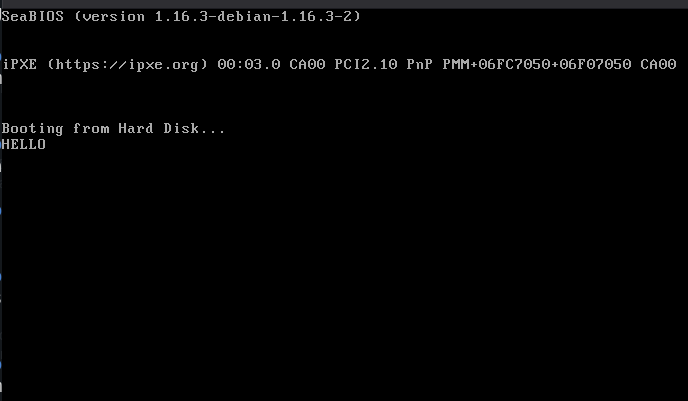
\includegraphics[width=0.5\textwidth]{images/bootloader_hello.png}
    \caption{Bootloader mostrando ``HELLO'' en QEMU.}
\end{figure}

\subsection{Conclusiones}

\subsubsection{Prueba en hardware real}

Una vez comprobado el funcionamiento del bootloader en entorno virtualizado, se procedió a grabarlo en un dispositivo USB físico y probarlo en una computadora real.

Los pasos realizados fueron:

\begin{enumerate}
    \item Conectar únicamente el pendrive para evitar confusiones con otros discos.
    \item Identificar el dispositivo correcto mediante el comando:
    \begin{lstlisting}[language=bash]
lsblk
    \end{lstlisting}
    \item Desmontar la partición montada del pendrive:
    \begin{lstlisting}[language=bash]
sudo umount /dev/sdc1
    \end{lstlisting}
    \item Grabar la imagen del bootloader en el dispositivo completo:
    \begin{lstlisting}[language=bash]
sudo dd if=main.img of=/dev/sdc bs=512 count=1 status=progress
    \end{lstlisting}
    \item Expulsar de forma segura el pendrive:
    \begin{lstlisting}[language=bash]
sudo eject /dev/sdc
    \end{lstlisting}
    \item Insertar el pendrive en la computadora de prueba, acceder al \textit{Boot Menu} durante el arranque (presionando F12, F10, ESC o la tecla correspondiente) y seleccionar el pendrive como dispositivo de arranque \textbf{en modo Legacy (no UEFI)}.
\end{enumerate}

Al bootear desde el pendrive, el sistema ejecutó correctamente el bootloader, mostrando el texto programado.

\begin{figure}[H]
    \centering
    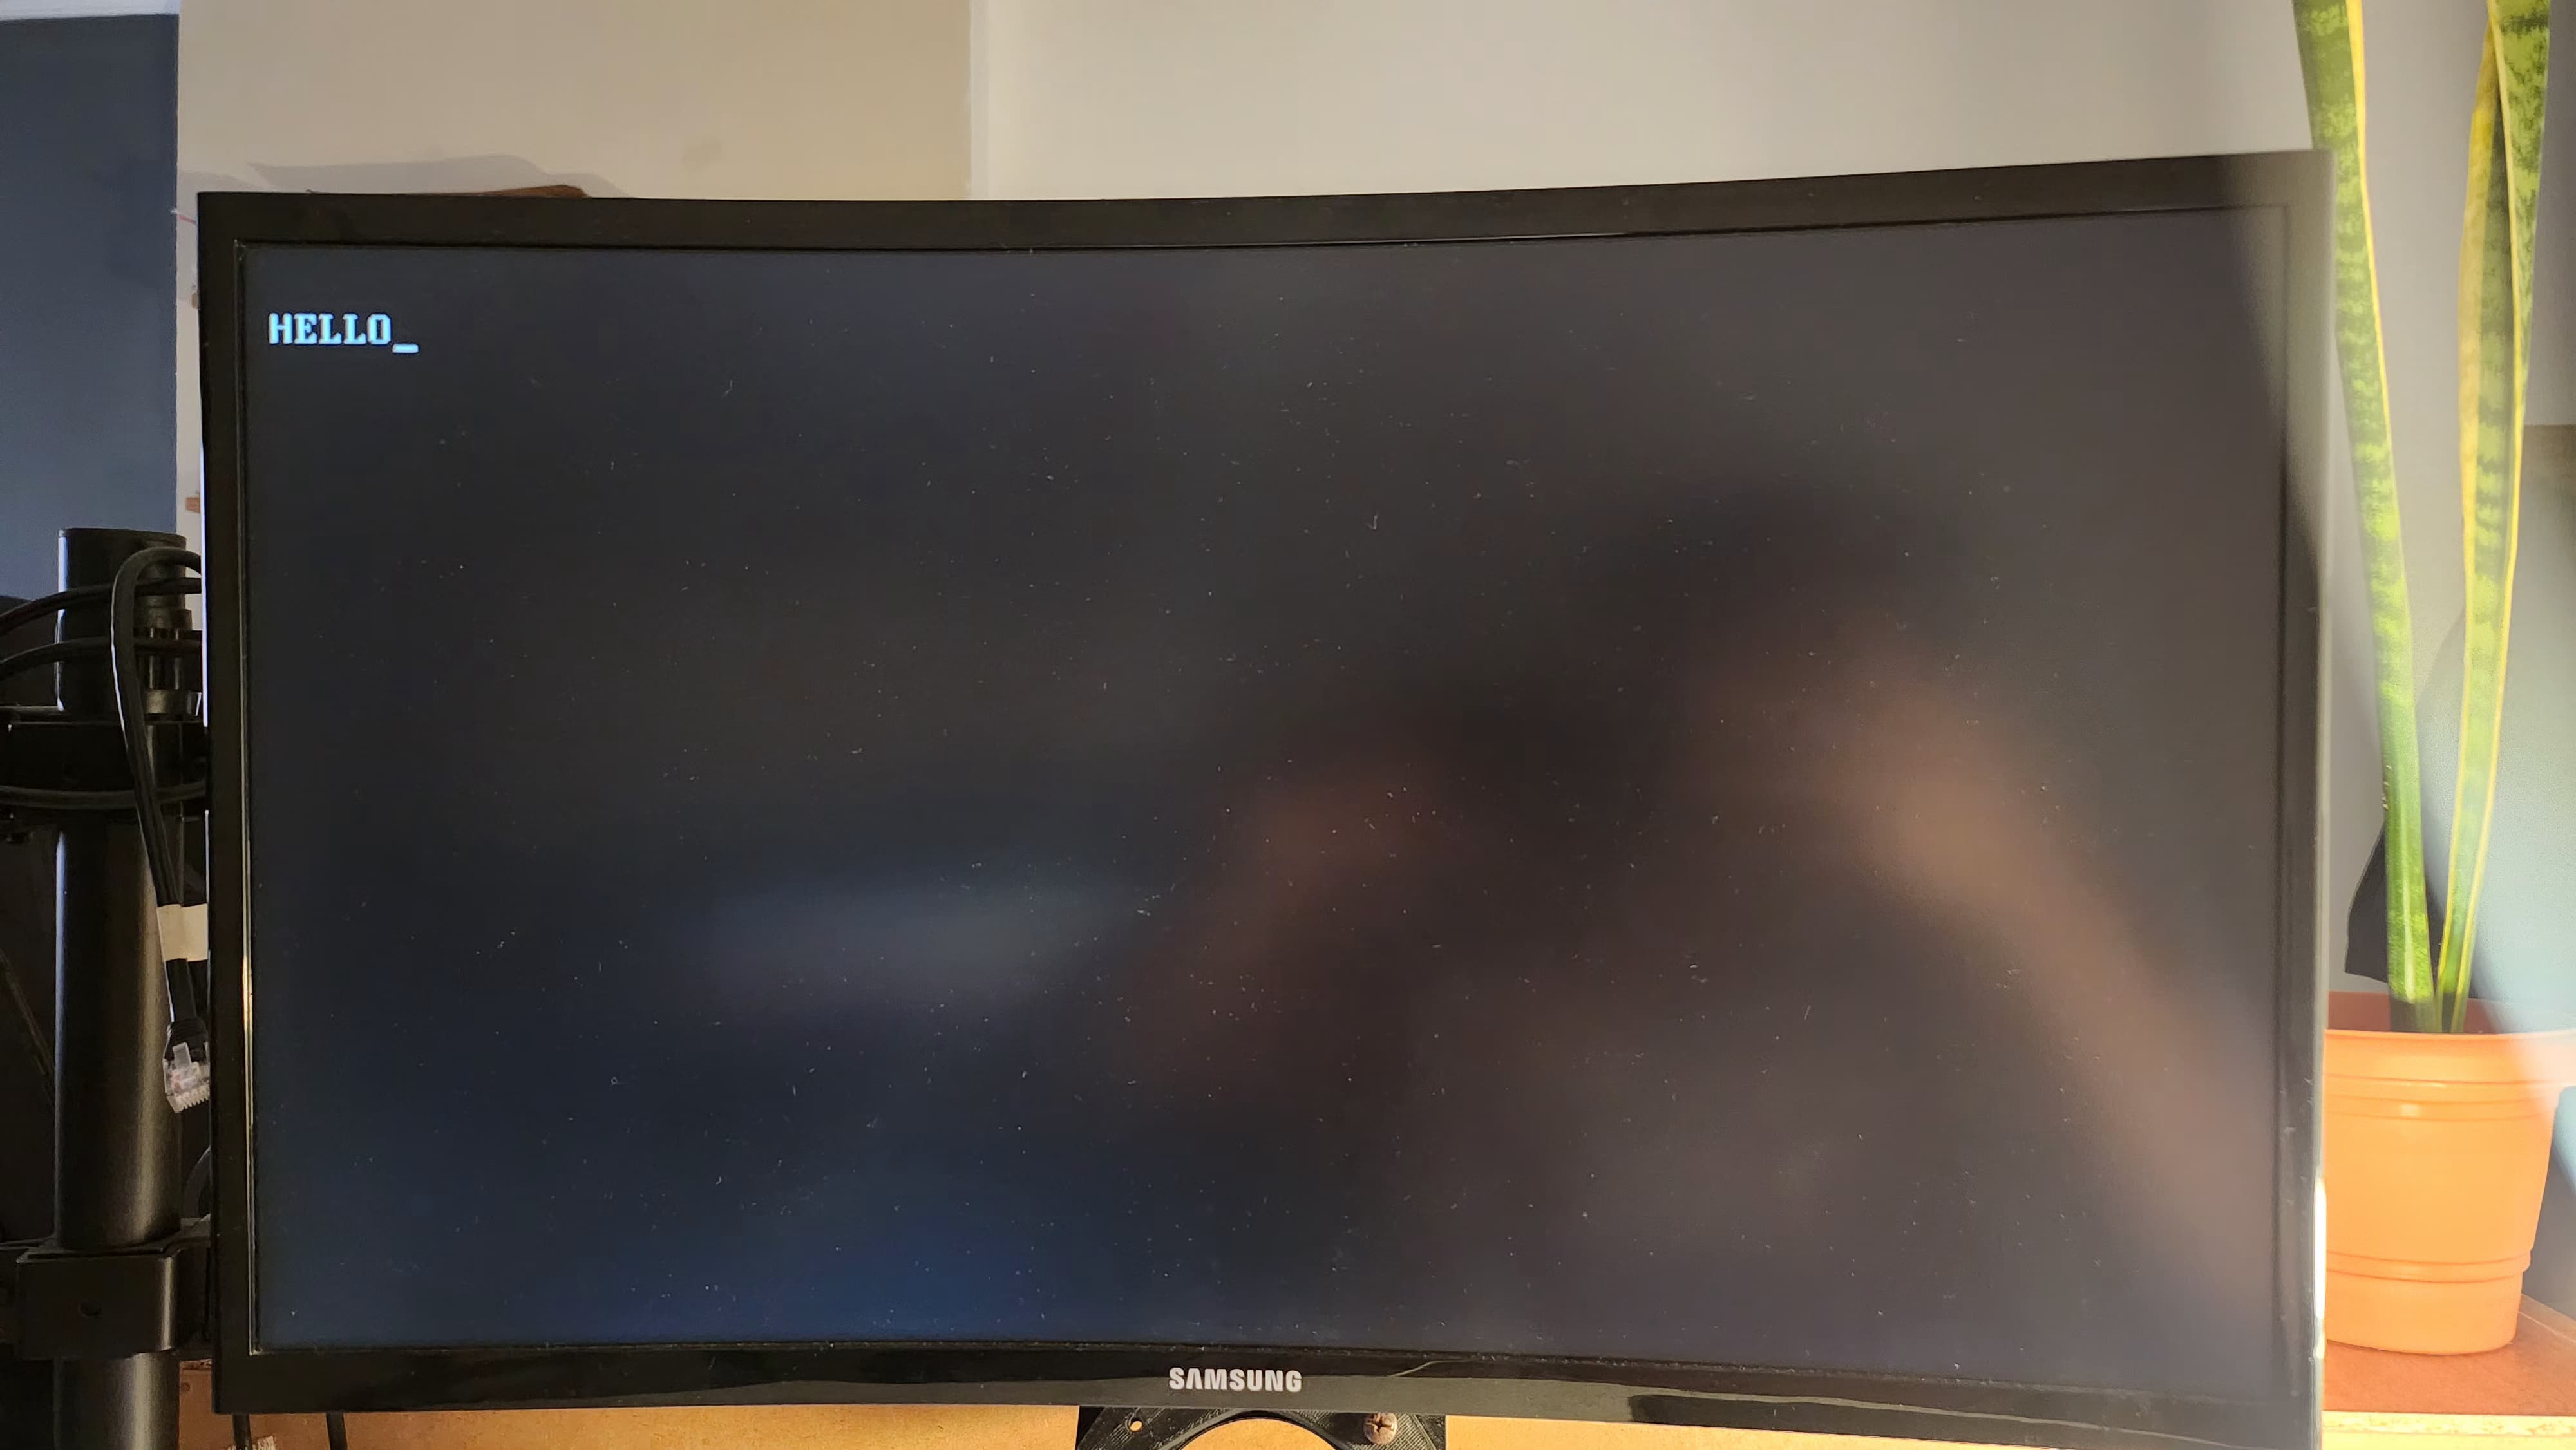
\includegraphics[width=0.5\textwidth]{images/bootloader_pendrive.jpeg}
    \caption{Bootloader mostrando ``HELLO'' desde pendrive en hardware real.}
\end{figure}

Esta práctica permitió:
\begin{itemize}
    \item Comprender el flujo de arranque de una PC desde nivel BIOS.
    \item Aplicar conocimientos de lenguaje ensamblador en un entorno de bajo nivel.
    \item Experimentar con herramientas de emulación de hardware.
\end{itemize}

Se consolidó así el conocimiento sobre cómo interactuar directamente con el hardware sin sistemas operativos intermedios.
